\documentclass[10pt,a4paper]{article}

%double si on veut une version prof et une version élève. simple si on veut une seule version.
\newcommand{\buildmode}{double}

\InputIfFileExists{version.tex}{}{}
% Version (définie par le script)
\providecommand{\version}{eleve}

\usepackage{feuilleactivite}

%%%à modifier à chaque fois

\renewcommand{\niveau}{1M}
\renewcommand{\chapitre}{Fonctions, généralités}
\renewcommand{\numchap}{0.1} 
\renewcommand{\theme}{Fonctions}

\begin{document}


%\legendeicones

\vspace{-0.3cm}

\begin{objectifs}
\begin{itemize}
    \item Lire et comprendre un graphique comme la représentation d'une fonction.
    \item Se réapproprier le vocabulaire des fonction.
    \item Lire et compléter un tableau de valeurs.
\end{itemize}
\end{objectifs}

\section{Courbe de température}

Le graphique ci-dessous représente l'évolution de la température en °C à Saint-Denis le 15 août 2026. 

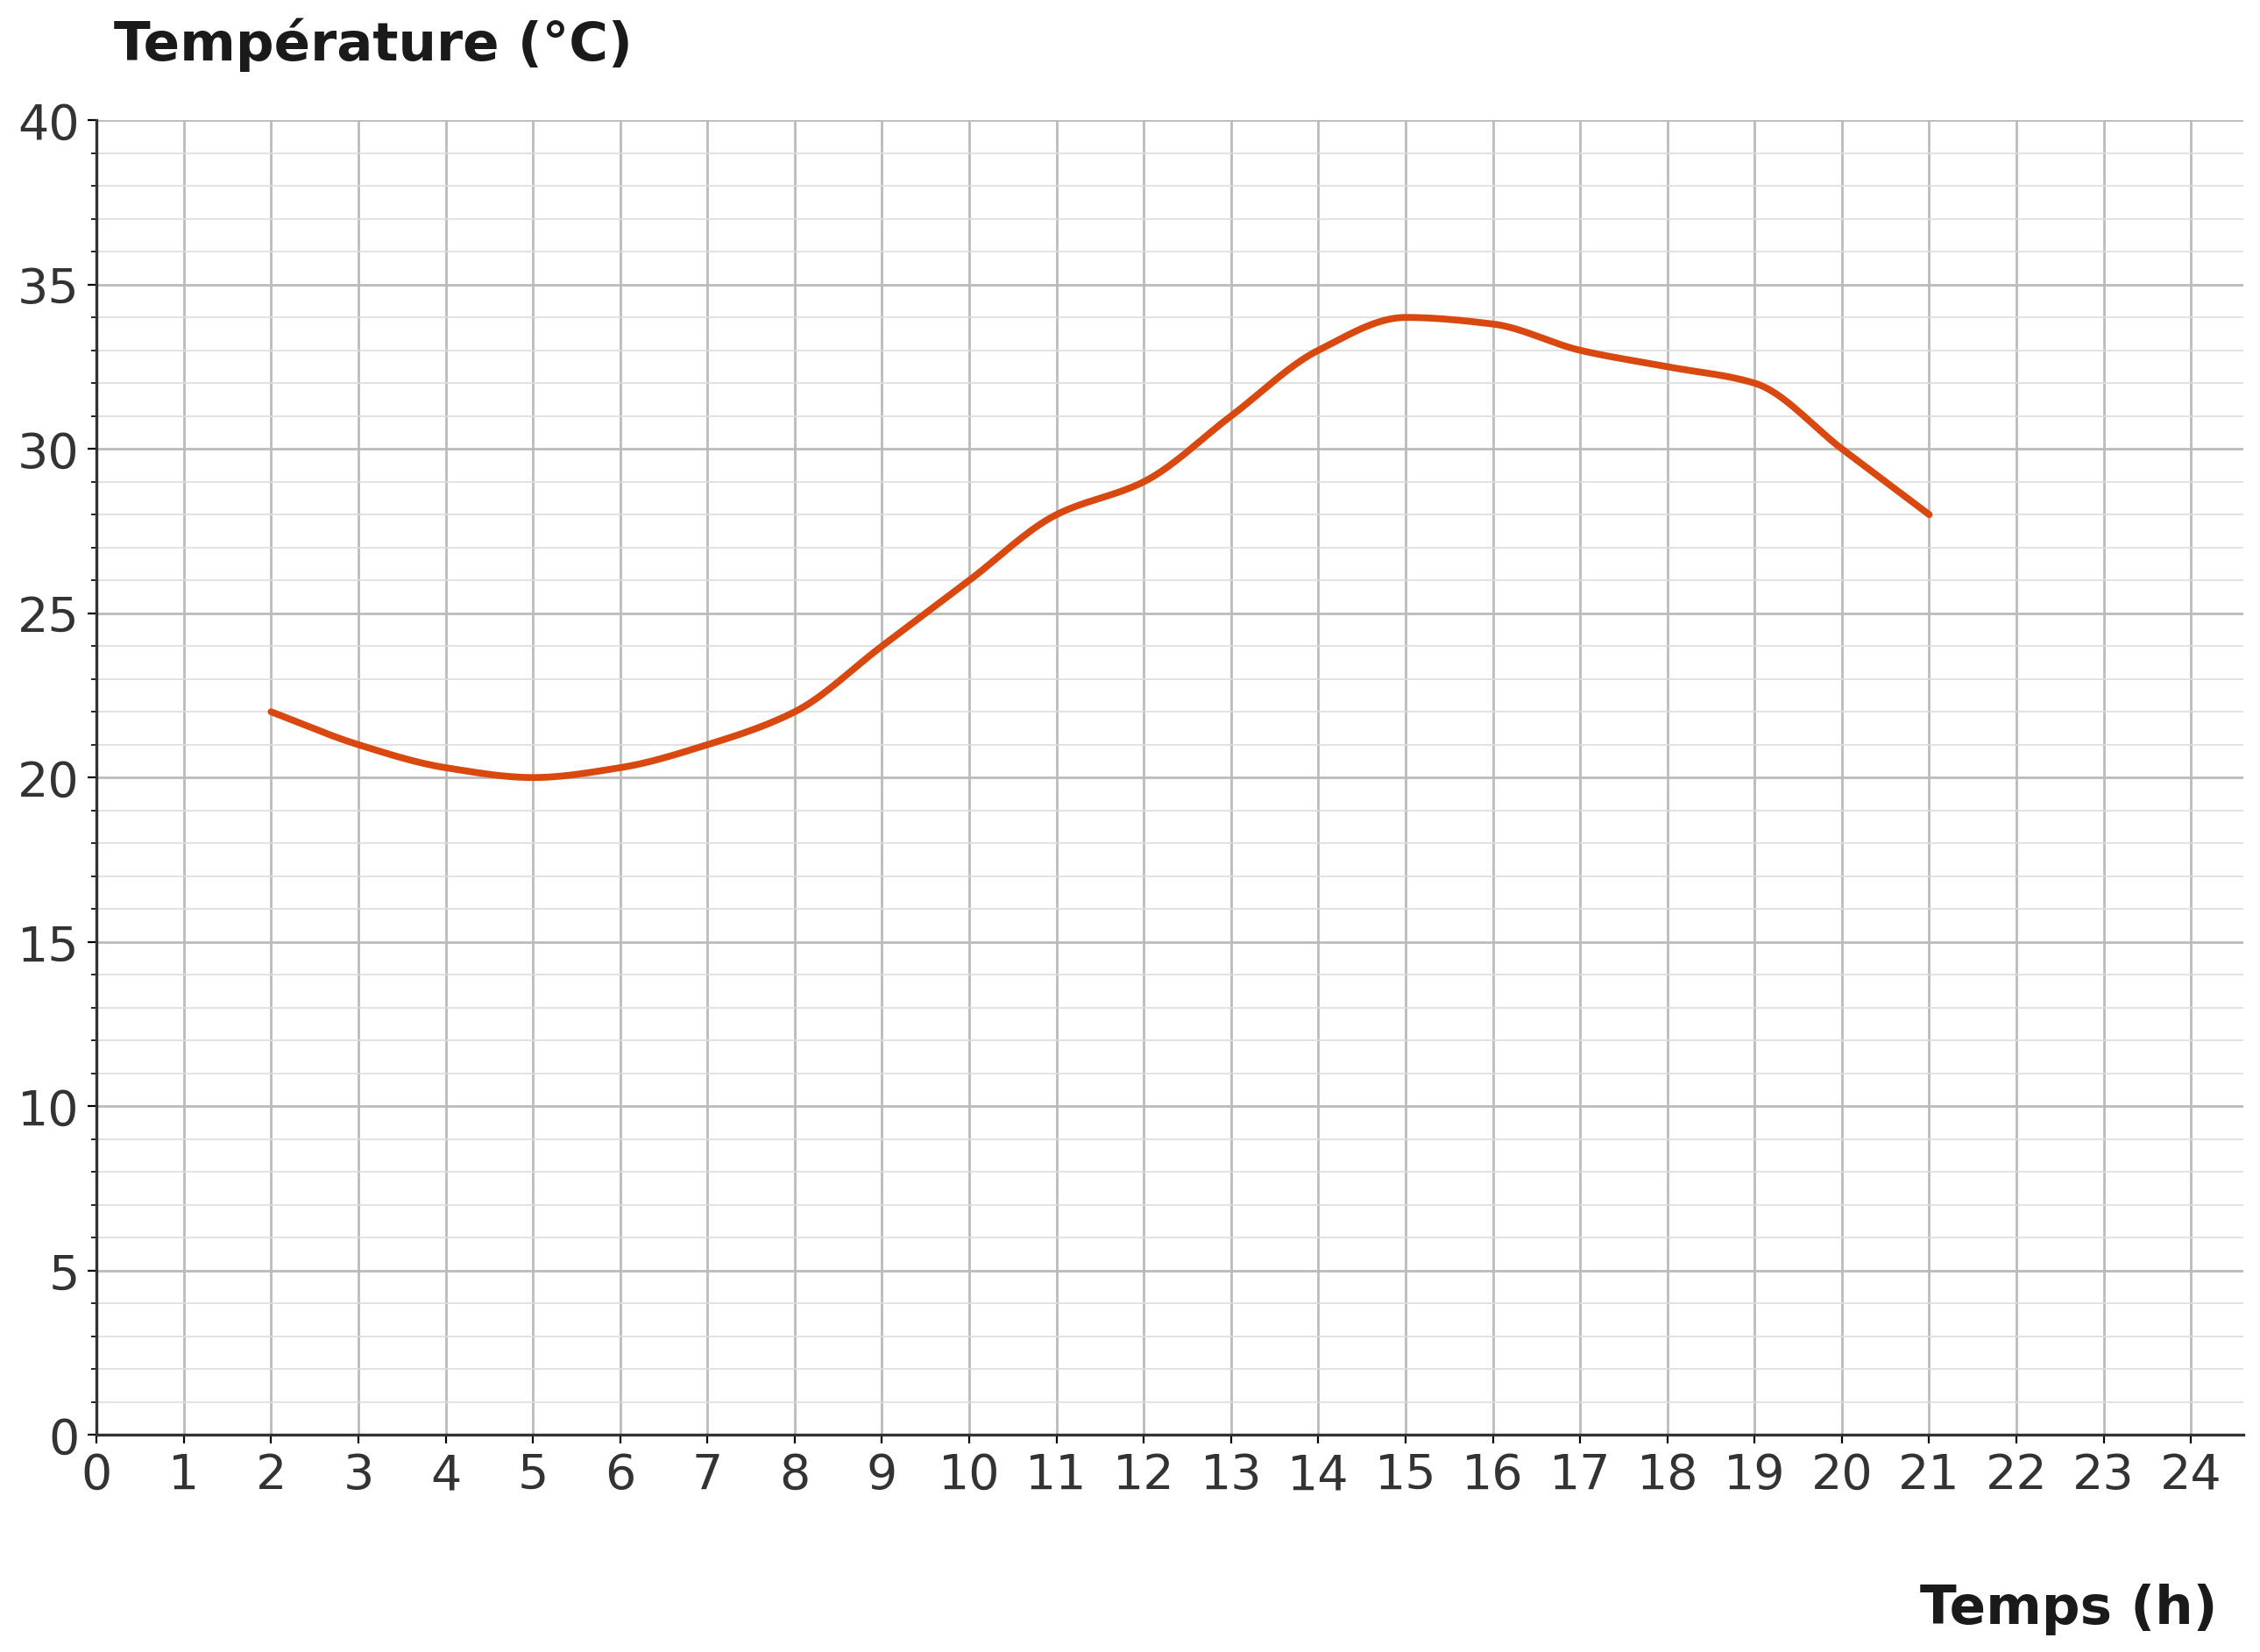
\includegraphics[width=0.8\textwidth]{saint_denis_93_temp_full_axis.png}

\begin{enumerate}

    \item Utilisez le graphique pour répondre aux questions suivantes :
    \renewcommand{\arraystretch}{2} %donne la distance entre les lignes%
    %\setlength{\tabcolsep}{1cm} %donne la distance entre les colonnes%
    \begin{center}
    \begin{tabular}{|p{5cm}|p{12cm}|}
    \hline
    Questions & Réponses \\
    \hline
    \hline
    Sur quels horaires les températures ont-elles été relevées ? & \\
    \hline
    Quelle était la température à 7h du matin ? &    \\
    \hline
    A quelles heures la température était-elle de 30°C ? &  \\
    \hline
    Sur quelles plages horaires la température a-t-elle diminué ? & \\ 
    \hline
    Entre 9h et midi, la température a-t-elle augmenté ou diminué ?& \\ 
    \hline
    Donner les températures extrêmes. A quelles heures ont-elles pu être observées ?  & \\
    \hline
    \end{tabular}
    \end{center}


    \item Listez tous les mots de vocabulaire dont vous vous souvenez de l'année de seconde sur les fonctions (par exemple : antécédent). 
    \prof{
        Mise en commun au tableau. On attend au moins : image, antécédent, ensemble de définition, croissant, maximum.

        Définir la fonction température avec les élèves et l'appeler \(f\). Réfléchir aux variables didactiques, \(t\) ou \(f\).
    }

    \medskip

    \textit{\underline{Commentaire :} On considérera maintenant que la température est une fonction du temps, que l'on notera \(f\)}

    \medskip


    \item Le tableau ci-dessous est le même que celui de la question 1, mais reformulé avec le vocabulaire des fonctions. Complétez-le.
    


        \begin{center}
    \begin{tabular}{|p{5cm}|p{12cm}|}
    \hline
    Questions & Réponses \\
    \hline
    \hline
    Quel est l'ensemble de définition de la fonction ? & L'ensemble de définition de la fonction est l'intervalle \([2\ ;\; 21]\) \\
    \hline
     Quelle est l'image de 7 par la fonction \(f\) ? &  \vspace{1cm}   \\
    \hline
    \vspace{1cm} &  \\
    \hline
    Sur quelles intervalles la température est-elle décroissante ? & \\ 
    \hline
    \vspace{1cm}  & La température est croissante sur l'intervalle \([9\ ; \ 12]\)  \\ 
    \hline
     \vspace{1cm} &  \\
    \hline
    \end{tabular}
    \end{center}
    
\end{enumerate}

\section{Tableau de valeur}
On considère la fonction \(f\) définie sur l'intervalle \([0\ ;\ 5]\) par \(f(x)=x^2-2x+3\). 


\begin{multicols}{2}
    \begin{enumerate}
    \item Complétez le tableau de valeurs suivant.
    \begin{tabular}{|c|c|c|c|c|c|c|}
    \hline
    \(x\) & 0 & 1 & 2 & 3 & 4 & 5 \\
    \hline
    \(f(x)\) &  &  &  &  &  &  \\
    \hline
    \end{tabular}

    
    \item Complétez le graphique suivant

    \end{enumerate}
\end{multicols}
\end{document}
